\documentclass[a4paper,12pt,reqno]{article}
\usepackage{styledoc19}

\addbibresource{references.bib}

\begin{document}

    \docNumber{RU.17701729.12.20-01 ПМИ 01-1}
    \docFormat{Программа и методика испытаний}
    \student{БПИ 213}{В. А. Андронов}
    \project{Веб-приложение для ведения лабораторных и вычислительных экспериментов с поддержкой онтологий\unskip}
    \supervisor{Доцент департамента \vfill программной инженерии \vfill факультета компьютерных \vfill наук, кандидат \vfill технических наук}{О. В. Максименкова}

    \firstPage
    \newpage
    \secondPage
    \newpage
    \thirdPage
    \newpage

    \section{Объекты испытаний}

    \subsection{Наименование программы}
    Веб-приложение для ведения лабораторных и вычислительных экспериментов с поддержкой онтологий (Ontologically-controlled data management of laboratory and computational experiments in chemistry and materials science\unskip)

    \subsection{Область применения программы}

    \subsubsection{Функциональное назначение}
    Разрабатываемое решение предоставляет возможность создавать, описывать, просматривать, редактировать и экспортировать эксперименты лабораторных и вычислительных экспериментов. Эксперименты описываются с привязкой к онтологиям из расширяемого набора возможных онтологий предметной области.

    \subsubsection{Эксплуатационное назначение}
    Приложение должно использоваться в лабораториях химии и материаловедения, в очередь РТУ МИРЭА. Конечными пользователями являются группы научных сотрудников, студенты, а также ML-разработчики и аналитики данных.

    \subsubsection{Краткая характеристика области применения}
    Онтологически-контролируемое управление данными представляет собой современный подход к систематизации и обработке информации в химии и материаловедении. Данный метод основывается на использовании онтологий — формальных описаний концепций и их взаимосвязей в конкретной предметной области, что позволяет создать единое семантическое пространство для обмена знаниями и данными~\cite{ontology:base}.

    В условиях увеличивающихся объемов данных и сложных междисциплинарных исследований, необходимость в эффективных инструментах управления информацией становится все более очевидной. Онтологически-контролируемое управление данными позволяет не только организовывать большие объемы информации, но и обеспечивать их интероперабельность. Это упрощает процессы интеграции данных из различных источников и способствует более тесному сотрудничеству между научными коллективами и организациями, занимающимися исследованиями в смежных областях.
    \newpage

    \section{Цель испытаний}
    Проверка на соответствие требованиям, указанным в документе <<Веб-приложение для ведения лабораторных и вычислительных экспериментов с поддержкой онтологий\unskip. Техническое задание>>.

    \section{Требования к программе}

    \subsection{Требования к к составу выполняемых функций}

    Система должна предоставить пользователю следующий набор функций:

    \begin{enumerate}
        \item Регистрация и аутентификация пользователей.
        \item Создание лабораторных и вычислительных экспериментов.
        \item Работа с таблицами результатов измерений.
        \item Привязка данных к онтологиям.
        \item Экспорт и импорт данных в JSON и CSV.
        \item Взаимодействие с API для управления экспериментами.
    \end{enumerate}

    \subsection{Требования к интерфейсу}

    Интерфейс пользователя должен поддерживать следующие возможности:
    
    \begin{enumerate}
        \item Регистрация и авторизация.
        \item Система навигации по экспериментам.
        \item Визуализация данных экспериментов.
        \item Форма ввода данных с привязкой значений к онтологиям.
        \item Поддержка адаптивного дизайна.
    \end{enumerate}

    \subsection{Требования к надежности}

    \begin{enumerate}
        \item Отказоустойчивость при возникновении любых некорректных API-запросов.
        \item Запись в журнал (лог) всех аварийных ситуаций для возможности разбора сбоев.
        \item Защита ресурсов от несанкционированного доступа за счет использования сессионной модели, идентификации пользователя и role-based access control~\cite{arch:RBAC}.
        \item Защита паролей пользователей за счет использования вместо них их криптографических хэшей.
    \end{enumerate}

    \section{Требования к программной документации}

    \subsection{Состав программной документации}
    Состав программной документации должен включать в себя следующие компоненты:
    \begin{enumerate}
        \item Техническое задание <<Веб-приложение для ведения лабораторных и вычислительных экспериментов с поддержкой онтологий\unskip>> (ГОСТ 19.201-78) \label{tz}
        \item Программа и методика испытаний <<Веб-приложение для ведения лабораторных и вычислительных экспериментов с поддержкой онтологий\unskip>> (ГОСТ 19.301-78) \label{pmi}
        \item Руководство оператора <<Веб-приложение для ведения лабораторных и вычислительных экспериментов с поддержкой онтологий\unskip>> (ГОСТ 19.505-79) \label{ro}
        \item Текст программы <<Веб-приложение для ведения лабораторных и вычислительных экспериментов с поддержкой онтологий\unskip>> (ГОСТ 19.401-78) \label{tp}
    \end{enumerate}

    \indent
    Вся документация должна быть составлена согласно ЕСПД (ГОСТ 19.101-77, 19.104-78, 19.105-78, 19.106-78 и ГОСТ к соответствующим документам (см. выше))~\cite{TZ:gost0, TZ:gost1, TZ:gost2, TZ:gost3, TZ:gost4, TZ:gost5, TZ:gost6, TZ:gost7, TZ:gost8, TZ:gost9, TZ:gost10, TZ:gost11}. Все документы сдаются в электронном виде в составе выпускной квалификационной работы LMS НИУ ВШЭ.

    \newpage

    \section{Средства и порядок испытаний}

    \subsection{Технические средства, используемые во время испытаний}
    Во время проведений испытаний использовался персональный компьютер со следующими характеристиками:
    \begin{enumerate}
        \item Операционная система: MacOS 15.3.2.
        \item ОЗУ 16 Гб.
        \item Тип системы: 64 разрядная.
    \end{enumerate}

    \subsection{Программные средства, используемые во время испытаний}
    Для проведения испытаний использовался браузер Google Chrome.

    \subsection{Порядок проведения испытаний}
    Испытания было проведены в следующем порядке:
    \begin{enumerate}
        \item Проверка требований к программной документации.
        \item Проверка требований к интерфейсу.
        \item Проверка требований к функциональным характеристикам.
        \item Проверка требований к надежности.
    \end{enumerate}

    \newpage

    \section{Методы испытаний}
    Испытания представляют собой процесс установления соответствия подсистем и программной документации заданным требованиям.

    \subsection{Проверка требований к программной документации}
    Состав программной документации проверяется визуально, проверяется наличие всех необходимых разделов и наличие программной документации в системе LMS. Также визуально проверяется соответствие документации требованиям ГОСТ. Все документы удовлетворяют представленным требованиям.

    \subsection{Проверка требований к функциональным характеристикам}

    \textbf{Тест 1: Регистрация нового пользователя}\\
    Шаги:
    \begin{enumerate}
        \item Открыть страницу регистрации.
        \item Ввести имя пользователя, пароль.
        \item Нажать кнопку "Зарегистрироваться".
    \end{enumerate}
    Ожидаемый результат: успешное создание учетной записи.

    \begin{figure}[H]
        \centering
        
\includegraphics[width=0.5\linewidth]{img/signup.png}
        \caption{Страница регистрации}
    \end{figure}
    \vspace{0.6cm}

    \textbf{Тест 2: Вход в аккаунт}\\
    Шаги:
    \begin{enumerate}
        \item Открыть страницу входа.
        \item Ввести имя пользователя, пароль.
        \item Нажать кнопку "Войти".
    \end{enumerate}
    Ожидаемый результат: успешный вход на основную страницу.

    \begin{figure}[H]
        \centering
        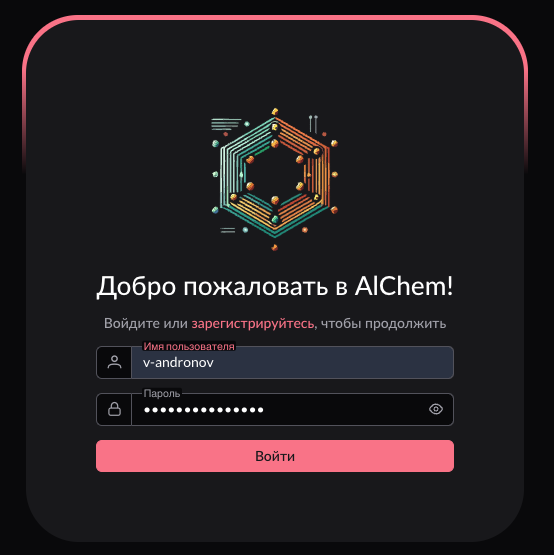
\includegraphics[width=0.5\linewidth]{img/signin.png}
        \caption{Страница входа}
    \end{figure}
    \vspace{0.5cm}

    \textbf{Тест 3: Создание папки}\\
    Шаги:
    \begin{enumerate}
        \item Войти в систему.
        \item Нажать кнопку "Создать", выбрать опцию "Папка".
        \item Ввести название папки и выбрать где она будет располагаться.
        \item Нажать кнопку "Создать".
    \end{enumerate}
    Ожидаемый результат: папка создана с правильным именем в нужном месте.

    \begin{figure}[H]
        \centering
        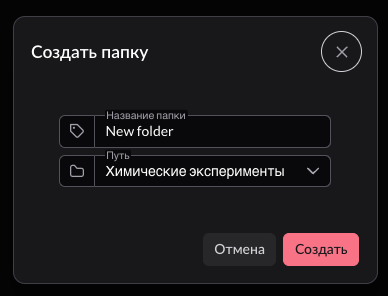
\includegraphics[width=0.5\linewidth]{img/create_folder_modal.png}
        \caption{Модальное окно создания папки}
        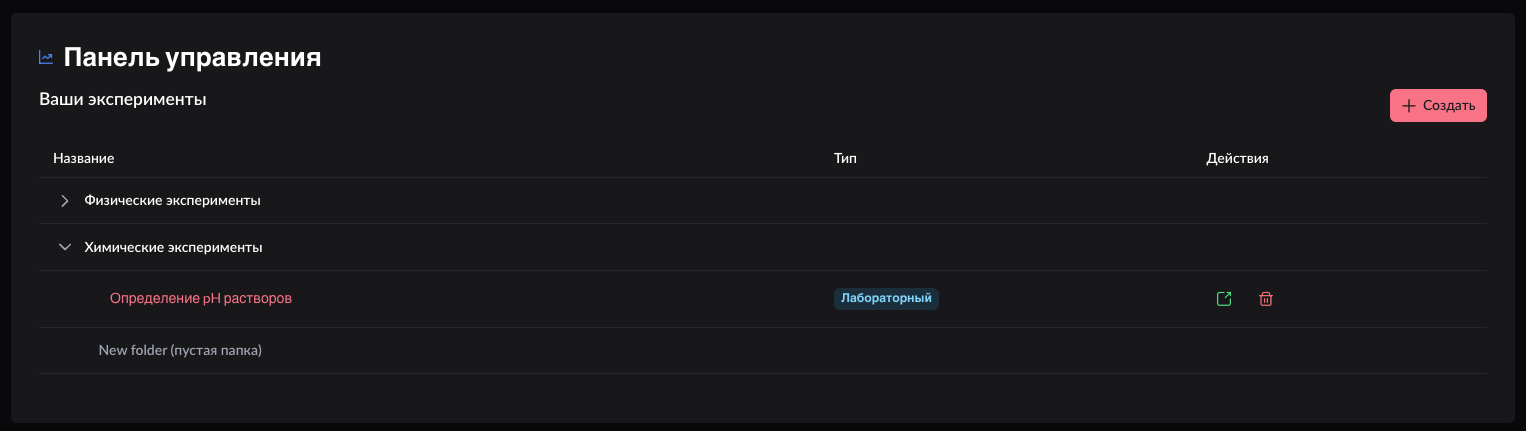
\includegraphics[width=\linewidth]{img/create_folder_result.png}
        \caption{Результат создания папки}
    \end{figure}
    \vspace{0.5cm}
    
    \textbf{Тест 4: Создание экспериментов}\\
    Шаги:
    \begin{enumerate}
        \item Войти в систему.
        \item Нажать кнопку "Создать", выбрать опцию "Эксперимент".
        \item Выбрать тип, ввести название эксперимента и выбрать где он будет располагаться.
        \item Сохранить эксперимент.
    \end{enumerate}
    Ожидаемый результат: эксперимент создан с правильным именем в нужном месте.

    \begin{figure}[H]
        \centering
        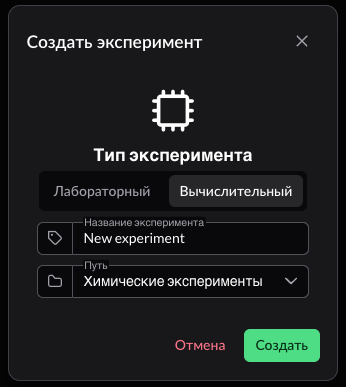
\includegraphics[width=0.5\linewidth]{img/create_experiment_modal.png}
        \caption{Модальное окно создания эксперимента}
        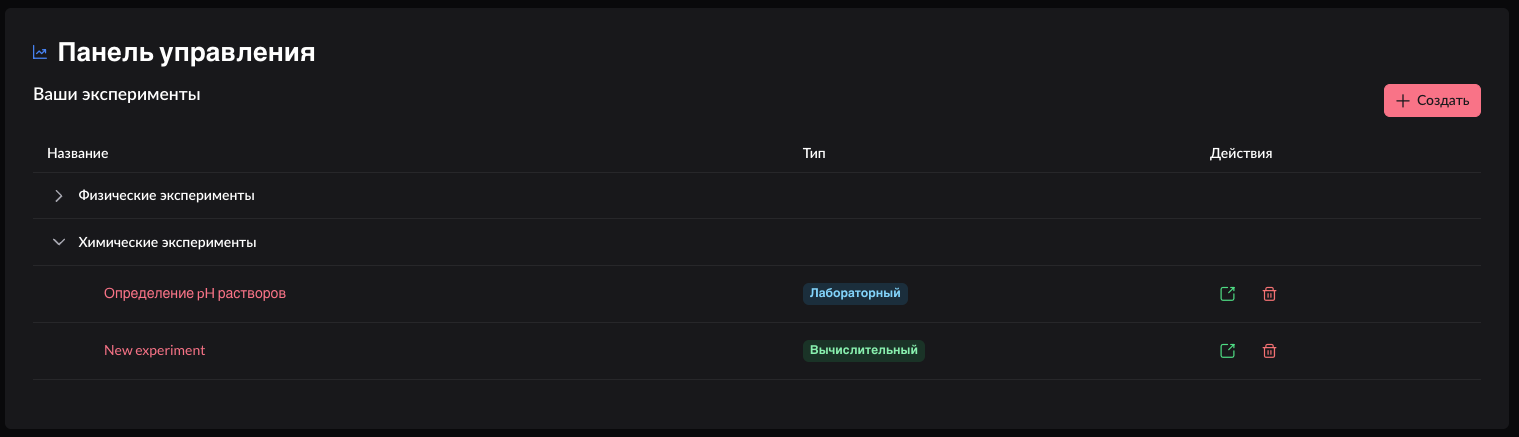
\includegraphics[width=\linewidth]{img/create_experiment_result.png}
        \caption{Результат создания эксперимента}
    \end{figure}
    \vspace{0.5cm}

    \textbf{Тест 5: Отображение дерева экспериментов}\\
    Шаги:
    \begin{enumerate}
        \item Войти в систему.
        \item Создать произвольное ненулевое количество экспериментов и папок.
    \end{enumerate}
    Ожидаемый результат: эксперименты корректно отображаются в папках.
    
    \begin{figure}[H]
        \centering
        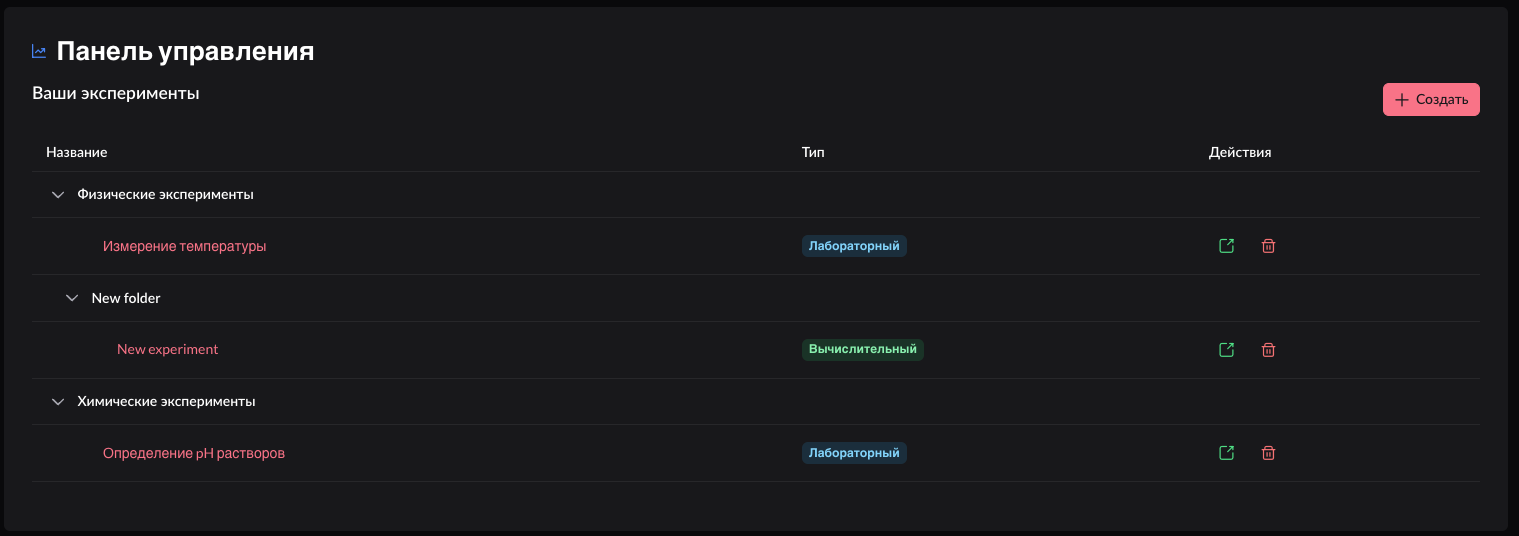
\includegraphics[width=\linewidth]{img/experiments_tree.png}
        \caption{Окно с деревом экспериментов}
    \end{figure}
    \vspace{0.5cm}

    \textbf{Тест 6: Просмотр данных эксперимента}\\
    Шаги:
    \begin{enumerate}
        \item Войти в систему.
        \item Открыть эксперимент.
    \end{enumerate}
    Ожидаемый результат: эксперимент корректно открывается, виден редактор описания и таблица с данными эксперимента.

    \begin{figure}[H]
        \centering
        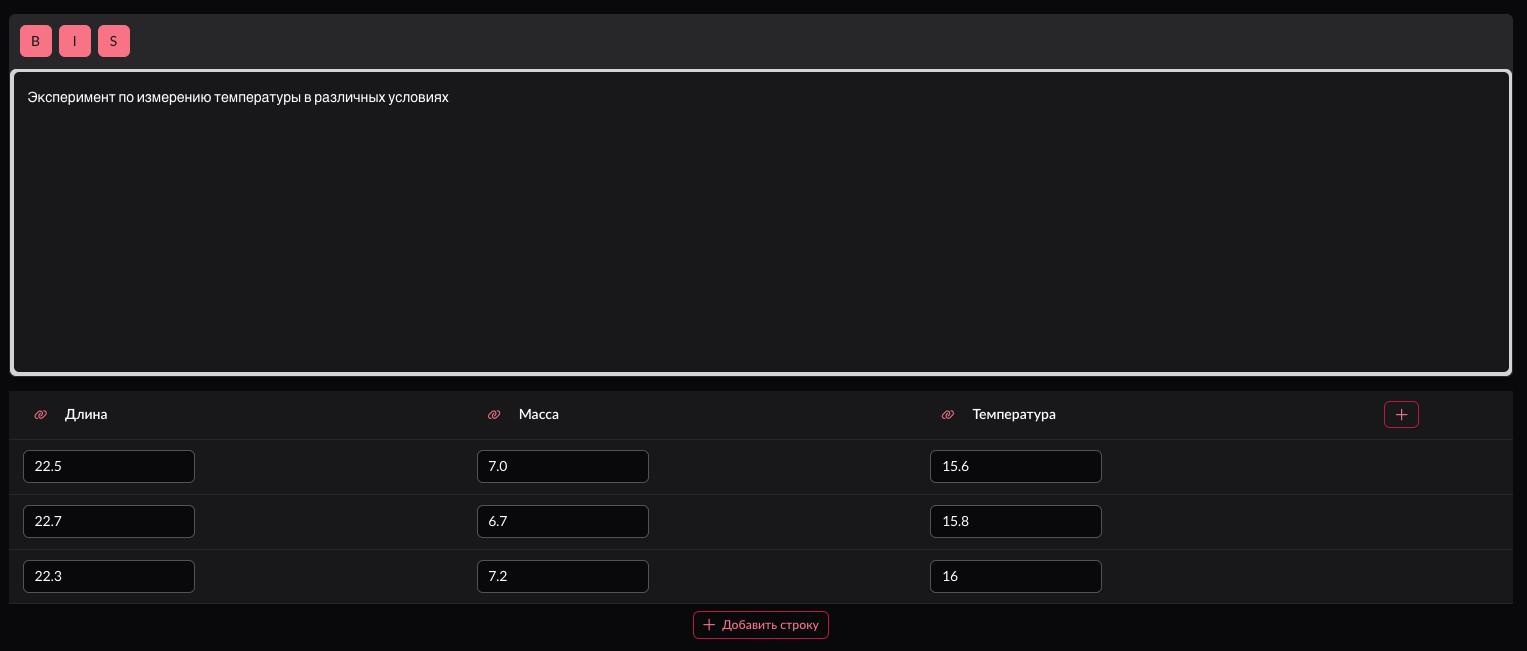
\includegraphics[width=\linewidth]{img/experiment_view.png}
        \caption{Окно просмотра данных эксперимента}
    \end{figure}
    \vspace{0.5cm}

    \textbf{Тест 7: Привязка столбцов к элементам онтологий}\\
    Шаги:
    \begin{enumerate}
        \item Войти в систему.
        \item Открыть эксперимент.
        \item Нажать на иконку рядом с названием любого столбца.
        \item Ввести название онтологии и уникальный идентификатор элемента онтологии, позволяющий отличить его от всех других.
        \item Нажать кнопку "Закрыть".
    \end{enumerate}
    Ожидаемый результат: при повторном нажатии на иконку рядом с названием столбца введённые данные должны сохраниться.

    \begin{figure}[H]
        \centering
        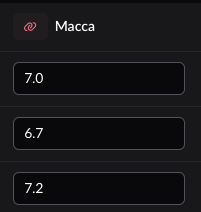
\includegraphics[width=0.5\linewidth]{img/ontology_column_pick.png}
        \caption{Выбор столбца для настройки онтологии}
        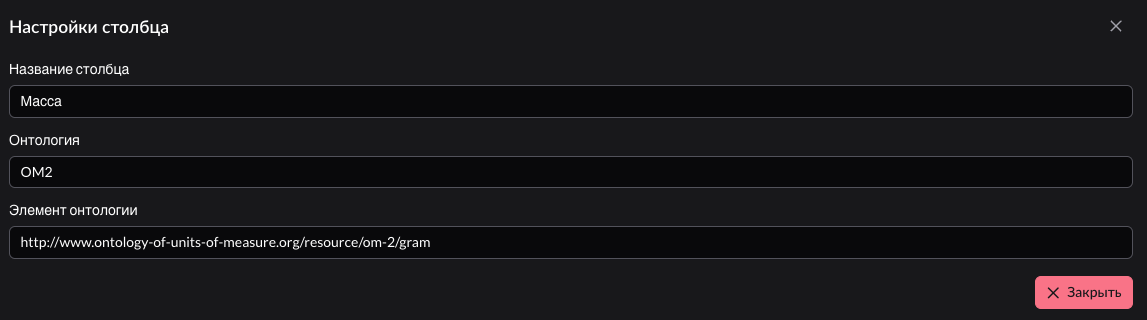
\includegraphics[width=\linewidth]{img/ontology_modal.png}
        \caption{Ввод данных об онтологии}
    \end{figure}
    \vspace{0.5cm}
    
    \textbf{Тест 8: Добавление строк}\\
    Шаги:
    \begin{enumerate}
        \item Войти в систему.
        \item Открыть эксперимент.
        \item Нажать кнопку "Добавить строку".
        \item Нажать кнопку "+" справа от всех столбцов.ещв
        \item Настроить новый столбец аналогично пункту 4 теста 7
    \end{enumerate}
    Ожидаемый результат: новые строка и столбец эксперимента корректно отображаются, при повторном нажатии на иконку рядом с названием нового столбца введённые данные должны сохраниться, новые ячейки доступны для редактирования.

    \begin{figure}[H]
        \centering
        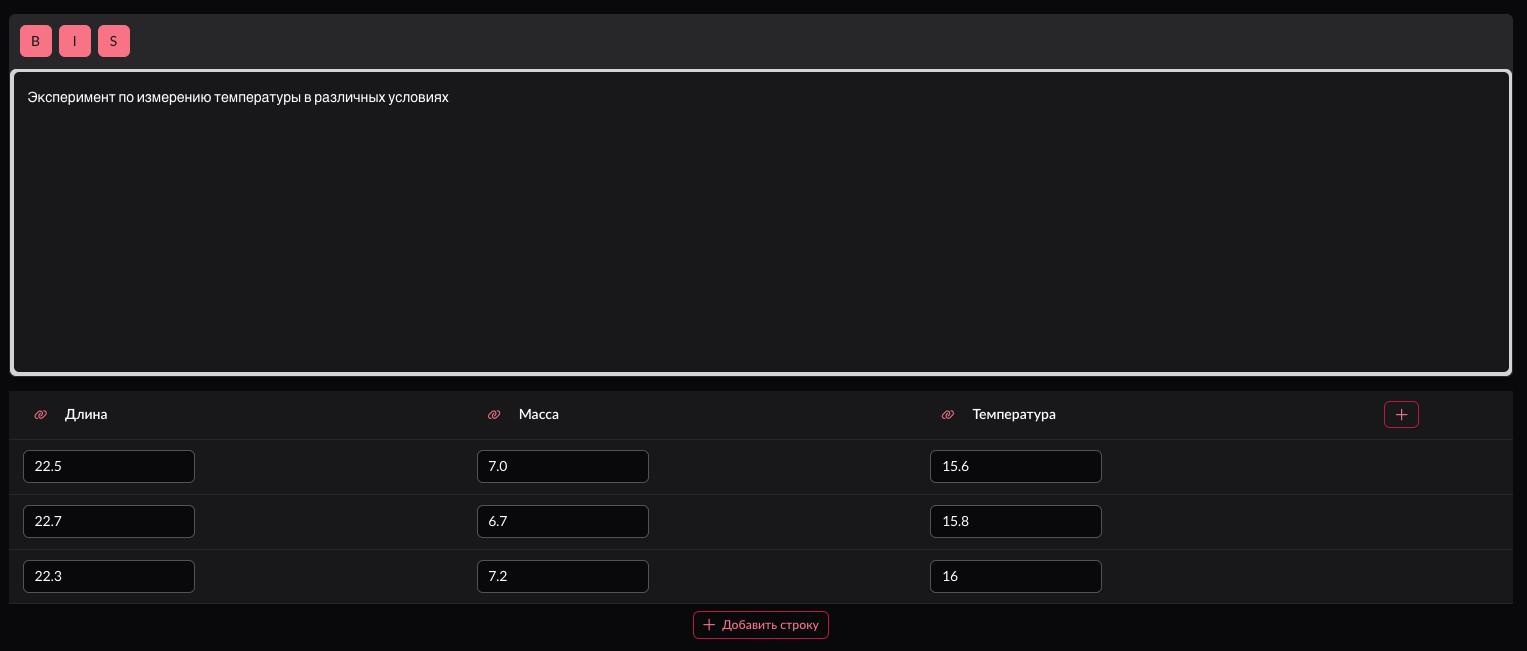
\includegraphics[width=\linewidth]{img/experiment_view.png}
        \caption{Окно просмотра данных эксперимента с нужными кнопками}
        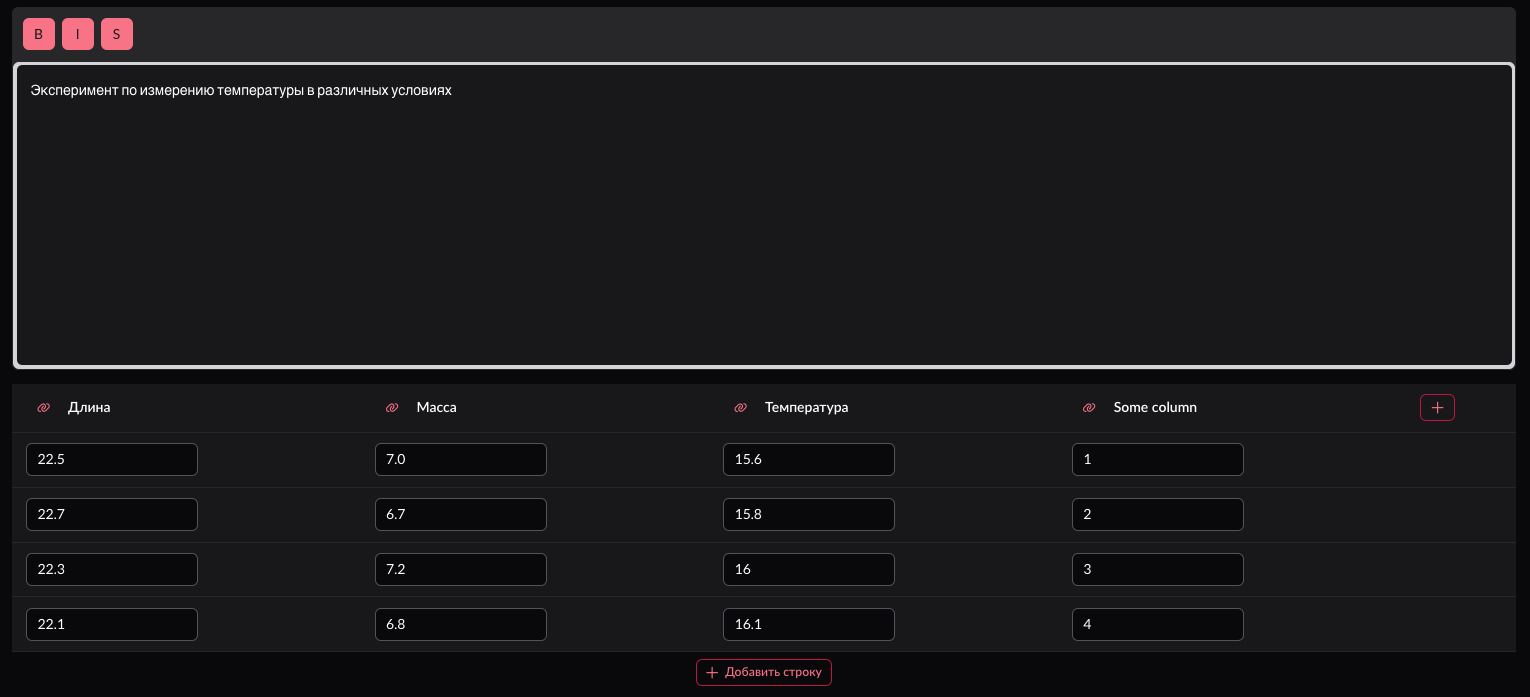
\includegraphics[width=\linewidth]{img/add_data_result.png}
        \caption{Результат добавления новых строки и столбца}
    \end{figure}
    \vspace{0.5cm}

    \subsection{Проверка требований к надёжности}

    Требование об отказоустойчивости удовлетворяется выбранным фреймворком FastAPI~\cite{Framework:FastAPI}, обеспечивающим перехват любых исключений в клиенстком коде без аварийного завершения сервера.

    \textbf{Тест 9: Хранение хэшированных паролей}\\
    Шаги:
    \begin{enumerate}
        \item Зарегистироваться согласно тесту 1.
    \end{enumerate}
    Ожидаемый результат: в базе данных должен появиться пользователь с указанными при регистрации данными и ролью RESEARCHER, но его пароль должен быть захэширован.

    \begin{figure}[H]
        \centering
        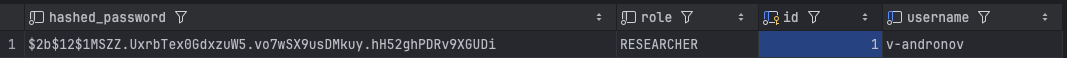
\includegraphics[width=\linewidth]{img/hashed_password.png}
        \caption{Результат регистрации с точки зрения базы данных}
    \end{figure}
    \vspace{0.5cm}

    \newpage
    \printbibliography[title=Список источников, heading=bibintoc]

    \newpage
    \listRegistration

\end{document}